
\chapter{系统设计}
\label{chap:design}

前面两章介绍了本系统的研究目的,要解决的问题和对于这些问题本系统提出的解决方案。虽然第二章中只简单提到了解决方案,而并没有涉及系统具体的逻辑结构。但是从第二章的介绍,也不难看出本文介绍的系统大概的系统架构与主要的功能设置。接下来的两章我们将深入的介绍该系统的逻辑结构和部分实现细节。下面将通过“统一接口”、“文档撰写与展示”、“用户空间逻辑结构”、“社交网络与门户”几个部分,逐步介绍本系统的逻辑结构。

\section{统一接口}
\label{sec:restful}

前文提到,本系统要实现的一个重要功能就是使用户文档可以方便的在不同种类的设备间传递,这些设备包括运行windows操作系统的PC机、运行mac操作系统的apple机、运行ios平台和android平台手机和平板电脑、运行linux操作系统的实验用机和各种移动阅读设备(电纸书)等等。显然,要实现这样的功能,就要求任何设备上的客户端程序都可以访问系统服务器上的数据,并且访问的方式要相对统一。这样才能尽可能的降低服务器端程序的复杂度,使系统结构尽量紧凑。

面向统一接口的web service服务架构,显然是实现如上功能的不二选择。web service的主要特点就是:客户端访问web service只需要通过因特网标准协议,如HTTP或XML。因为HTTP协议和XML都是与平台无关的标准协议,因此,可以被任何主流操作系统正确理解和解释。

web service的常用的方法有:
\begin{enumerate}
\item RPC 所谓的远程过程调用 (面向方法):像调用本地服务(方法)一样调用服务器的服务(方法),通常的实现有XML-RPC,JSON-RPC,通信方式基本相同, 所不同的只是传输数据的格式。
\item SOA 所谓的面向服务的架构(面向消息):前几年炒的很火的一个词, SOA是基于消息的,通常与具体的实现语言无关, 所以在一定程度上得到大公司的支持。
\item REST 所谓的 Representational state transfer (面向资源):是以资源为中心, 名词即资源的地址, 动词即施加于名词上的一些有限操作, 表达是对各种资源形态的抽象。
\end{enumerate}
本系统选择架构比较清晰,可扩展性较好,也是目前被广泛提倡使用的REST结构。REST 是英文 Representational State Transfer 的缩写,是近年来迅速兴起的,一种基于 HTTP,URI,以及 XML 这些现有协议与标准的,针对网络应用的设计和开发方式。它可以降低开发的复杂度,提高系统的可伸缩性。REST 的核心是可编辑的资源及其集合,用符合 Atom 文档标准的 Feed 和 Entry 表示。每个资源或者集合有一个惟一的 URI。系统以资源为中心,构建并提供一系列的 Web 服务。REST 的基本概念和原则包括:系统上的所有事物都被抽象为资源、每个资源对应唯一的资源标识、对资源的操作不会改变资源标识本身、所有的操作都是无状态的等等。

在 REST 中,开发人员显式地使用 HTTP 方法,对系统资源进行创建、读取、更新和删除的操作:
\begin{enumerate}
\item 使用 POST 方法在服务器上创建资源
\item 使用 GET 方法从服务器检索某个资源或者资源集合
\item 使用 PUT 方法对服务器的现有资源进行更新
\item 使用 DELETE 方法删除服务器的某个资源
\end{enumerate}

图~\ref{fig:xfig9}所示为本系统基本的结构图。从图中我们可以看到的基本信息有:
\begin{enumerate}
\item 本系统是以B/ S为基本架构的。
\item 本系统提供基本的WEB用户界面供用户使用,用户可以在任何有浏览器的环境中访问系统,撰写和获取自己的文档资源。
\item 除了以WEB为主的浏览方式以外,系统还提供了标准的Restful的API接口,通过该接口系统可以直接为各种操作系统,甚至移动设备中的本地程序(APP)提供数据。也就是说,用户不仅可以通过浏览器访问本系统,也可以通过安装本地客户端程序访问系统。
\end{enumerate}
通过以上几点,我们不难发现,由于本系统架构设计上的合理。使本系统天生具有很高的开放性。开放Restful的API接口的好处不仅是为用户访问系统提供了方便,更深层次的意义在于。任何组织和个人都可以利用统一接口来编写程序访问本系统中的数据\footnote{当然,这需要一定的授权}。这也就意味着,不管是学校还是第三放组织,在制作其他系统是需要用到教师和学生的文档数据时,就不需要再重新收集和存储,可以通过和本系统的无缝集成来直接获取这些数据。这给老师和学生带来的方便也是不言而喻的,他们起码不用把自己的数据在办理不同业务时重复的整理和提交。只要把这些数据存放到本系统中就可以了。同时我们的数据也不再是信息孤岛,他们可以被搜素引擎检索到\footnote{当然,这是在用户愿意公开的前提下},并通过文档自身的价值引起更多人的关注。

顺便提一下,其实当今,Restful的API接口的应用已经非常流行,大到 google,yahoo等大公司在自己的系统是使用这样的服务,小到刚刚起步的国内的一些小的互联网公司也在做这方面的探索。所以我个人认为,封闭的,自称体系的信息管理系统(erp)的时代已经过去了,取而代之的是以统一接口为驱动的。开放性的网络服务系统。通过开放的接口,和完善的授权机制,我们可以建立更加开放,更加安全,也更加实用的系统。关于统一接口的话题我们就先进行到这里,在系统实现的章节里我们将详细描述本系统的Restful API接口。
\begin{figure}[H]
  \centering
  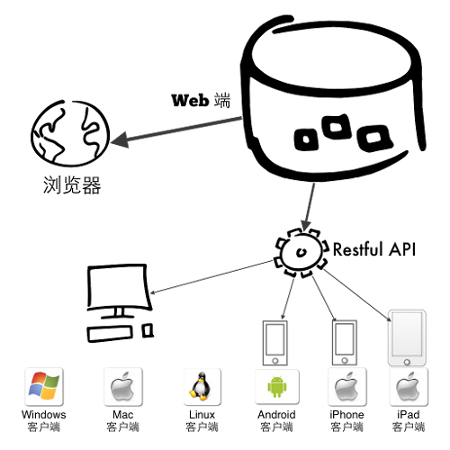
\includegraphics{restful}
  \caption{系统提供web端和restful api接口结构图}
  \label{fig:xfig9}
\end{figure}
通过以上介绍,我们看到,通过系统的统一接口设计从根本上解决了高校用户个人文档管理中不同设备间存取难和不同步的问题,同时也解决了用户在不同场合需要文档数据时,重复整理、重复提交的问题。但是有的时候用户的文档并不满足于自己存取和管理,有的时候我们的用户希望自己的文档可以分发给别人,甚至请别人修改自己的文档。或者和其他人一起合作完成文档。这就需要系统提供一定的社交功能和协作功能。我们将在下面的章节详细讲述本系统社交性和写作性的设计。



\section{文档的撰写与展示}
\label{sec:writeandview}

本系统鼓励用户使用\smarkdown在系统内直接撰写文档,但是考虑到用户的使用习惯不会在段时间内改变,所以系统在用户文档的设计部分,充分考虑到了word用户可以轻松上手的功能,首先系统提供了和Word操作很相似的富文本编辑页面与\smarkdown互为补充,用户可以按照自己的喜好选择自己喜欢的编辑环境。其次系统还提供了Word等格式文档的上传与预览功能。以满足Word用户的需要。

如图~\ref{fig:xfig10}所示,用户在系统中即可以使用\smarkdown格式书写文档,也可以使用富文本方式。用户可以在编辑页面直接插入图片,系统数据库会保存用户文档数据和相应的图片文件,然后通过转换成html格式进行预览。由于本系统是用户个人文档管理功能为主的系统,所以系统默认的文档浏览权限都是私有的,也就之只用用户本人可以浏览与编辑\footnote{文档编辑和浏览权限将在社交功能小节描述}。除此以外,系统可以把保存的数据通过格式转换引擎转成\LaTeX格式的文档并可以导出。还可以进一步生成为最终的PDF文档并导出。那么就实现了,用户只关心自己的文章内容,而文章的格式则有系统预设的多种格式的模板来自动设置。常用的格式模板都以\LaTeX格式模板形式提供,用户文档和模板的组合生成都在服务器端完成,用户不用安装任何软件也不用做任何的繁琐配置。只要对\smarkdown的简单语法略有了解,就可以完成科技论文等格式要求严格的文档的写作。并直接获取到最终排版好的的PDF文档。当然,如果用户对\LaTeX格式有一定了解的话,也可以在书写\smarkdown文本的时候添加\LaTeX语法片段。这样就可以更精细的控制文档的格式。系统将陆续提供各大主流院校的毕业论文格式模板,和国内外知名出版社要求的期刊论文格式模板,以满足高校用户写论文的要求。用户只要在导出论文最终文档时 选择要导出的文档格式模板,那么就可以获取到相应格式最终文件,和文档的内容完全无关。这样也带来了另外一个好处,用户无需修改自己的文档,就可以轻松的把自己的文章转投到多家出版社。如果使用Word编辑工具是完全做不到的。\footnote{如果用户使用富文本方式书写文档那么,导出\LaTeX和使用模板生成PDF文档功能将不可用,但是对于初级用户用来编写个人博客和笔记还是非常够用的。}
\begin{figure}[H]
  \centering
  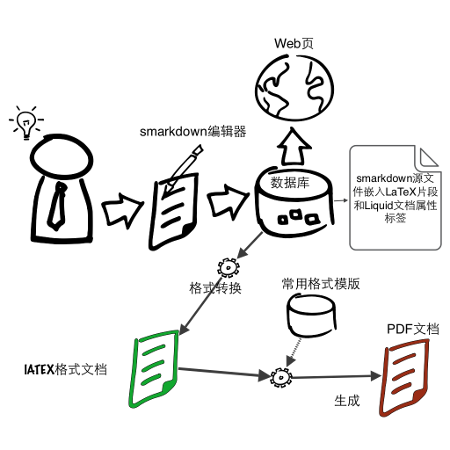
\includegraphics{writing}
  \caption{}
  \label{fig:xfig10}
\end{figure}

此外,系统在文档撰写功能部分还提供了。基本的版本控制功能,用户在建立文档时,可以定义此文档是否使用版本控制。如果使用,用户的每一次提交改变都会记录到系统,并且用户可以把文档恢复到任何一次提交以前的状态。但是每次修改文档都需要手动提交,并写明提交注释,所以建议在撰写重要的科技文档和书籍是使用。如果不使用,则系统不会保存文档的历史版本,文档的改变及时生效,定时保存。建议在笔记,博客等不重要的文档中使用。

\section{用户空间逻辑结构}
\label{sec:personstructure}

上文中曾经批评过Windows操作系统的文档管理中目录结构松散,与缺乏标签管理等问题。那么,本系统中的文档组织又是什么样的呢? 如图~\ref{fig:xfig11}所示,显然,本系统的文档组织也是由目录组成。但是这里的目录的概念和window操作系统中的目录概念不太一样。本系统的文档组织有如下特点:
\begin{enumerate}
\item 每一篇文档都隶属一个目录。
\item 每篇文档都由文档内容和若干文档属性组成,在编辑文档内容的时候,可以插入文档属性到内容中。文档显示的时候,插入的文档属性可以以用户选取的方式显示在文档中。文档有哪些属性由用户自定义\footnote{系统会预设一些常用的属性列表}。
\item 隶属于一个目录中的文档具有相同的属性,该属性列表由目录属性设定。每个目录需要定义一个属性列表。并定义属性的必要选项,比如必填,选填等。
\item 每个目录还必须设定一个文档默认显示方式,对于只有属性没有内容的文档。将使用目录中定义的默认模板显示属性。
\item 每个目录可以设定一个目录的首页模板,也就是用户访问该目录文档列表的时候显示的页面。系统将预设一些常用的页面,用户也可以自己定义。
\item 如果每个目录都从头自定义属性,那么使用起来会非常不方便。所以系统提供了目录继承功能。也就是新建目录的时候可以选择一个已有的目录继承,继承的内容包括属性列表、默认内容模板,目录首页模板等。目录继承可以使用强制和非强制的方式,强制继承方式要求子目录不可以删除父目录定义的属性,但是可以增加自己的属性。非强制继承不要求子目录一定设置父目录属性,只在建立时复制了父目录的属性。\footnote{目录继承不限于个人空间内,也可以通过目录继承共享继承其他用户的目录结构后面的章节将介绍。}
\end{enumerate}

不难看出,比起相对松散的windows系统的文件管理,文档在本系统中的组织形式更加严密,结构也更加复杂。如此设计的目的在于借助系统级的某些强制约定来帮助用户形成规范的文档管理习惯。每个目录中的文档必须有相同的属性在某种程度上强制用户把某一类内容很相近的文档放到同一个目录中。而文档中可以插入属性的功能,保证了文档内容的灵活性与规范性的平衡。而目录的继承功能则保证了系统即可以被配置成功能复杂的信息管理系统,也可以通过非常简单的方式提供给刚刚使用系统的用户使用。以上描述获取不能清楚的表达设计用意,下面举几个简单的例子:
\begin{itemize}
\item 假如目录A如此设置:文档属性只保留一个“任意文件类型”属性,目录的首页模板使用资源管理器模板,文档默认显示模板为显示文件内容。文档内容页留空。那么目录A就变成了一个网络磁盘应用。
\item 假如目录B如此设置:文档属性只保留一个“图片文件类型”属性,目录的首页模板使用图片幻灯片模板,文档默认显示模板为显示图片内容,文档内容页留空。那么目录B就变成了一个云端相册应用。
\item 假如目录C如此设置:文档属性设置为空,目录的首页模板使用文档摘要列表,文档默认显示模板为空。文档内容页我们可以写我们的文章,那么目录C就变成了一个网络日志应用。
\end{itemize}
综上所述,本系统即可以为初级用户提供简单的,易于使用的常用功能,这些功能不需要用户对系统有任何了解也可以无障碍的使用。又可以为高级用户提供十分复杂而强大的,具有极强的可配置性的高级功能。熟练使用本系统的用户可以使用本系统段时间内完成一个功能复杂的数据管理系统。

有一些编程经验的读者通过以上的描述可能已经发现了,本系统的目录和文档的结构设计与面向对象的编程的思想及其类似。系统中的目录就相当于面向对象系统中的类,而文档就相当于面向对象系统中的对象。属性就相当于面向对象系统中的属性。唯一缺少的是对象方法。由于本系统为文档管理系统。所以之需要文档为我们保存信息,而不需要做什么其他的事情,所以自然并不需要额外的方法。当然如果读者愿意,把文档的内容,目录的首页模板等理解为对象方法和类方法也完全可以。

以上多次提到文档属性,那么到底可以定义那些种文档属性呢?下面简单说明一下系统提供哪些类型的文档属性:
\begin{itemize}
\item 整数
\item 浮点数
\item 布尔值
\item 枚举值
\item 短字符串,纯文本
\item 大段字符串,纯文本
\item 大段字符串,富文本(\smarkdown)
\item 任意类型文件
\item 制定类型文件(Word,PDF,EXCEL等)
\item 图片
\item 视频
\item 链接
\item 表格数据
\item 日期时间
\item 数学公式,化学式,电路图等特殊专业的编辑器属性(\LaTeX格式)
\end{itemize}
除此意外还有一些高级的系统属性:
\begin{itemize}
\item 认证属性。此属性的功能将在后面小节详细介绍。
\item 由其他属性计算出结果的编程字段。\footnote{此功能计划使用R语言作为扩展语言,由于功能复杂度可能较高并不在目前版本中实现}
\end{itemize}
系统属性类型将随着系统的更加深入的使用,逐渐积累完善。以实现完整的系统生态环境。
\begin{figure}[H]
  \centering
  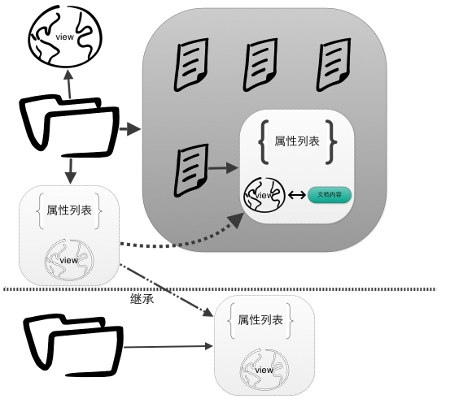
\includegraphics{person_s}
  \caption{用户空间逻辑结构}
  \label{fig:xfig11}
\end{figure}

当然,为来让用户更快上手使用系统,系统不会给用户直接提供一个“空壳”让用户自己建立目录结构。系统预设会给每个用户提供一个初始的目录结构。一方面,用户可以很快上手使用系统的常用功能,而无需花时间去了解系统中复杂的配置。另外一个方面,系统提供的预设的目录也是高级用户日常使用系统最常使用的部分。系统预设的目录包括:
\begin{description}
\item[我的简历] 存放用户的个人简历,由特定组织用户进行认证。
\item[我的成果] 主要保存用户完成的学术成果,包括发表的期刊论文,会议论文等。此目录结构继承自图书馆的一个共享目录,用户插入到此目录的文档可以申请图书馆的文献信息补全,和文献认证服务。
\item[我的著作] 主要保存用户编著的书籍。
\item[我的毕业论文] 针对学生用户,存放他们的毕业论文。此目录结构也继承自图书馆的一个共享目录,用户插入到此目录中的文档可以申请毕业论文提交服务。
\item[我的笔记] 可以添加用户笔记,此目录中的文章默认访问权限为私有。
\item[我的博客] 可以添加用户博客,此目录中的文章默认访问权限为公开。
\item[我的参考文献] 保存用户的参考文献,此目录也继承自图书馆的一个共享目录,图书馆提供参考文献信息服务。用户可以直接从图书馆目录中获取参考文献信息,并且可以导出多种格式,在用户使用\smarkdown撰写文章的时候,可以直接从该目录下选取文献,进行添加。省去了调整参考文献格式的时间。
\item[撰写中论文] 在该目录下,用户可以编写自己的科技论文,也可以通过继承该目录来自己定义章节书写论文。
\end{description}
以上为系统预设的一些目录,由于有些目录为学院业务必须。所以预设目录用户无权删除。用户也可以自己定义目录,以及通过继承预设目录来完成更多个性化配置。

另外,前文一直提到的标签体系也在本系统中得以实现,系统中的每一篇文档都可以被用户定义某些标签,这些标签既可以通过系统提供的预设列表中选取,也可以由用户自己定义。有了标签系统的帮助,用户可以很方便的查找自己的文档。不过标签系统,在本系统不叫“标签”这个名字,而是叫做“主题(Topic)”,系统将根据标准的专业和研究领域预设一个主题树供用户使用。关于主题将在下一节继续讨论。

\section{社交网络与门户}
\label{sec:society}

作为一个网络时代的信息系统,如果没有社交网络功能是怎么也说不过去的。所以社交网络也是本系统的一个功能特点,也是本系统区别于其他校园信息系统的一个重要特色。如上文所述,使用本系统,用户可以方便的在自己的多个设备中共享个人文档,并可以利用系统方便的撰写科技文献。但是,用户有时并不满足于孤立的保存文档。有时,用户希望可以把自己的文档方便的分发给自己的学生或者工作伙伴,也有的时候用户可能希望自己的某些文档可以在网络上被任何人访问到,可以被搜索引擎搜索到。设置有的时候用户可能希望和自己的项目组成员一起合作完成文档。要实现这些功能就需要系统拥有完备的社交网络和门户功能。下面就分别就“组织结构和用户认证”、“主题与分类”、“好友与关注”、“系统门户”、“个人门户与评论”、“用户组与圈子”、“目录共享和信息服务”、“用户邀请和提及系统”等几个方面分别介绍系统的社交网络功能。

\subsection{组织结构和用户认证}
\label{sec:auth}

本系统面对的用户为高校的教师和学生,所以系统用户信息需要包括用户的所属的学校、学院和专业等信息。也就是说系统用户基本上是以实名制登录系统。系统提供用户认证功能来确保用户个人信息的真是性。所以,系统管理中不需要为用户发文的信息审查问题担心\footnote{中国的信息审查制度确实是开放系统的天敌,实名制的系统要承担的责任要小很多。}。为用户搭建组织结构带来的另外一个好处是,在系统公共首页(总门户)中可以根据用户所在的学院专业快速导航到用户的个人空间和直接浏览某学院或专业中所有公开的文档。

用户认证机制,本系统将使用用户自己注册并由特定组织用户进行认证的方式和OAUTH认证协议\footnote{一种流行的获取统一用户信息的协议,通过该协议用户可以通过安全的方式获取到其他公共系统的用户信息,比如现在很多网站上的以qq,或者微博身份登陆的功能就是使用该协议。}的方式相结合。组织结构将分成三级 学校,学院,和专业,所以用户注册的时候只需填写用户名,密码,姓名,唯一标示(教师的工资号,学生的学号)和所属的单位信息即可。其余用户信息,比如性别,年龄等都被定义在用户的简历文档目录中的文档中。简历文档目录是一个预设目录,限制只能建一篇文档,该文档保存用户个人信息,并存在认证字段。

\subsection{主题与分类}
\label{sec:topic}

本系统的每一个文档都可以被标示上若干标签,标签的作用是标示此篇文档与哪些主题相关。标签可以由用户自己填写,填写的过程中系统会根据系统已有的标签进行提示。如果系统中已经有了相同的主题,用户可以直接选择。

系统建立只初,按照标准的学科与研究领域,预设了大量与各专业相关的主题。主题系统可以帮助用户快速的检索到自己的文档,也可以帮助系统浏览者快速的浏览到自己感兴趣的主题文档和导航到相关专家的个人空间。

为了减少用户为文档录入主题的操作。系统的目录可以设定默认主题,目录下的所有文档会自动填写上目录所设定的主题。

\subsection{好友与关注}
\label{sec:friend}

添加好友是一个社交系统的必备功能,近年来,随着微博等系统的流行,关注其他用户也成为了很多系统流行的功能,如果某用户follow了某个其他用户,那么该用户发布的任何有权限浏览的文档都会自动的推到该用户的管理首页上。比如,github就具有这样的功能。

所以本系统将同时支持添加好友,和follow用户功能。添加后的用户将放入用户的通讯录中。在用户撰写文档,分发文档的时候可以直接从通讯录中选取。follow后的用户文档,将自动发布在管理界面的首页。但是,本系统毕竟是一个文档管理系统,而非以社交交流为主的系统,所以目前系统并不提供微博系统中常用的转发,评论转发等功能。用户交流可以通过文档评论功能,和私信功能完成。

\subsection{系统门户}
\label{sec:golbal}

本系统结构设计采用分布式建库模式,为每一个系统用户(老师与学生)建立自己的存储空间,用户可以自己管理自己的空间,并提交(上传)数据,也可以由图书馆提供的资源建设服务或者信息认证补全服务来为用户提交标准的数据。发布端即可以通过用户的个人门户进行浏览检索,也可以通过,机构库统一的发布页面进行统一的浏览与检索。
